\documentclass[conference]{IEEEtran}
\usepackage{amsmath}
\usepackage{graphicx}
\usepackage{subcaption}
\usepackage{booktabs}

\title{A Second-Order PDE-Inspired Learnable Architecture for Image Denoising}

\author{
\IEEEauthorblockN{C V Rishi \hspace{3cm} G Rithvik}
\IEEEauthorblockA{
CSE, Mahindra University \hspace{3cm} CSE, Mahindra University \\
se23ucse044@mahindrauniversity.edu.in \hspace{3cm} se23ucse199@mahindrauniversity.edu.in
}

\vspace{0.3cm}

\IEEEauthorblockN{V Vivardhan \hspace{3cm} P Sai Sastha}
\IEEEauthorblockA{
CSE, Mahindra University \hspace{3cm} CSE, Mahindra University \\
se23ucse006@mahindrauniversity.edu.in \hspace{3cm} se23ucse141@mahindrauniversity.edu.in
}
}

\begin{document}

\maketitle

\begin{abstract}
We introduce a second-order partial differntial equation (PDE) image denoising model, which incorporates damping and inertial dynamics, that can be learned. In this approach, a more complicated evolution equation is introduced, which exhibits a hyperbolic character. Unlike first-order diffusion-based models such as Trainable Nonlinear Reaction Diffusion (TNRD), it is not based on diffusion. We use finite differences to break the PDE into smaller parts and then map those parts to a multi-stage unrolled network. We use learned convolutional filters with fixed influence functions in this network to simulate the diffusion operator. This model is trained in a greedy and stage by stage method with constant parameters. Experimental results on images contaminated by additive Gaussian noise demonstrate that our approach achieves a PSNR of 26.29 dB on the CBSD68 dataset, highlighting the utility of second-order dynamics.\end{abstract}

\begin{IEEEkeywords}
Image denoising, partial differential equations, second-order dynamics, TNRD, unrolled neural networks, Gaussian noise
\end{IEEEkeywords}

\section{Introduction}

Image Denoising is among the basic problems of image processing, in which the goal is to obtain a clean image based on the observations contaminated by noise. The main
problems are to eliminate noise and retain significant 
important features like edges and fine textures are present.
for visual quality.

PDE-based techniques have been applied to address partial Differential Equation (PDE) problems 
been popularly employed in image denoising because of their capability 
to approximate the diffusion process. Classical models such as
non-linear anisotropic diffusion are diffusion functions based 
to flatten area homogenously without changing the edges.
Nevertheless, they are hand-made, have to be manually tuned 
of parameters and functions which limits their performance
on various datasets and noise levels.

To overcome such constraints, diffusion models based on learning 
have been introduced. The example of one such outstanding example is the 
Trainable Nonlinear Reaction Diffusion (TNRD) framework \cite{chen2016tnrd},
where the denoising step is a multi-stage diffusion 
learnable parameters system. Both, linear filter and influence functions are learnt on the data, permitting the model in order to perform on a high level and remain efficient across datasets.

With these developments, the majority of the available diffusion-based models, such as TNRD, are based on first-order PDEs, in which the time dependence of the image is only dependent on its state. These type of formulations can be restrictive to the capability of the model to capture more complicated evolution behaviour when denoising process.

In this work, we consider a second-order PDE formulation for image denoising \cite{majee2020telegraph}, given by
\begin{equation}
u_{tt} + \gamma u_t = \operatorname{div}(c(|\nabla u|)\nabla u),
\end{equation}

This equation adds the inertial and damping effects to the process of diffusion, and permitting the evolution to be dependent on both the current and previous states of the image. We solve the suggested PDE with the help of finite difference schemes and consider the obtained update equations as an interpretation multi-stage architecture. The process of diffusion is applied using convolutional filters, and the model is trained in a
stage-wise fashion, in which specific parameters are chosen, like the influence and damping coefficient are constant, and the other parameters are learned on data.

\subsection{Contributions}

The main contributions of this work are:
\begin{itemize}
\item We suggest a second-order (hyperbolic) PDE-based formulation to image denoising, which is used to add inertial dynamics. 
\item We obtain a discretization based on finite differences and project it onto a stage-wise learnable architecture.
\item We model a training strategy in which influence functions and damping are parameters that are determined, and other parameters are learned.
\item We give a structural comparison with the TNRD model, pointing out the essential variations in dynamics and memory.
\end{itemize}

\section{Background}

\subsection{PDE-Based Image Denoising}

Partial differential equations (PDEs) have been widely used in image processing due to their ability to model diffusion processes. One of the most well-known models is the nonlinear anisotropic diffusion introduced by Perona and Malik \cite{perona1990}, which is given by

\begin{equation}
    \frac{\partial u}{\partial t} = \operatorname{div}(g(|\nabla u|)\nabla u),
\end{equation}
where $u$ represents the image, and $g(\cdot)$ is a diffusivity function that controls the amount of smoothing.

\subsection{Trainable Nonlinear Reaction Diffusion (TNRD)}

Learning-based approaches such as Trainable Nonlinear Reaction Diffusion (TNRD) \cite{chen2016tnrd} have been proposed to improve upon the performance for the general PDE-based image denoising.
\begin{equation}
u^{t} = u^{t-1} - \sum_{i=1}^{K} K_i^T \phi_i(K_i u^{t-1}) - \psi(u^{t-1}, f),
\end{equation}
where $K_i$ are linear filters, $\phi_i$ are influence functions, and $\psi(\cdot)$ represents a reaction term based on the observed noisy image $f$.

The advantage of TNRD is that both the filters and influence functions are learned from training data.

\section{Proposed Model}

\subsection{Second-Order PDE Formulation}

In contrast to conventional diffusion models based on first-order dynamics, we take into account a second-order partial differential equation for image denoising \cite{majee2020telegraph}, which is,
\begin{equation}
u_{tt} + \gamma u_t = \operatorname{div}(c(|\nabla u|)\nabla u),
\end{equation}
where $u$ represents the image, $u_t$ and $u_{tt}$ are the first and second-order time derivatives, and $\gamma$ is the dampening. The function $c(\cdot)$ controls the diffusion process and depends on the magnitude of the gradient.

\subsection{Discretization}

Where $u^t$ denotes stage $t$ image. The time derivatives can be approximated as
\begin{equation}
u_t \approx u^t - u^{t-1}, \quad
u_{tt} \approx u^t - 2u^{t-1} + u^{t-2}.
\end{equation}

Substituting these approximations into the PDE:
\begin{equation}
u^t = (2 - \gamma)u^{t-1} - (1 - \gamma)u^{t-2} + \operatorname{div}(c(|\nabla u^{t-1}|)\nabla u^{t-1}).
\end{equation}

This update equation shows that the current state depends not only on the previous state but also on the state before that.

\subsection{Learnable Diffusion Operator}

To make the model trainable, we replace the diffusion term with a learned operator. Specifically, the gradient and divergence operations are approximated using convolutional filters. The update rule can be written as
\begin{equation}
u^t = (2 - \gamma)u^{t-1} - (1 - \gamma)u^{t-2} - \sum_{i=1}^{K} K_i^T \phi(K_i u^{t-1}),
\end{equation}
where $K_i$ are learnable convolutional filters and $\phi(\cdot)$ is a fixed influence function.

\section{Training Strategy}

\subsection{Stage-wise Training}

We are using a greedy, stage-wise strategy. Each stage is trained one by one instead of all at the same time. At stage $t$, the parameters in that stage are optimized while keeping the parameters of previously trained stages fixed.

\subsection{Parameter Constraints}

The influence function $\phi(\cdot)$ and the damping coefficient $\gamma$ are kept constant across all stages. Only the convolutional filters are learned from data.

\subsection{Loss Function}

The model has been trained using the mean squared error (MSE) loss. Given a noisy input image $f$ and its corresponding clean image $u^*$, the loss is defined as
\begin{equation}
\mathcal{L} = \frac{1}{2} \| u^T - u^* \|^2,
\end{equation}
where $u^T$ denotes the output of the final stage.

\subsection{Training Details}

Training is performed on grayscale images corrupted with additive Gaussian noise with fixed noise level $\sigma$. It is trained for a fixed number of epochs per stage, and the parameters are optimized using standard gradient-based methods.

\section{Experiments}

\subsection{Datasets}

For training, we used the FOE400 dataset, which contains a diverse set of grayscale images. For evaluation, we used the CBSD68 dataset, which is a standard benchmark for image denoising.

\begin{figure*}[t]
\centering
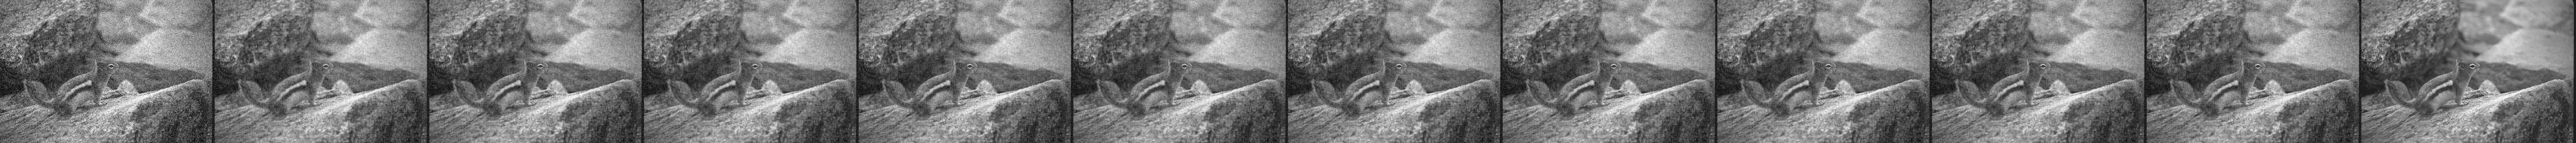
\includegraphics[width=\textwidth]{images/0000_stages.png}
\vspace{1em}
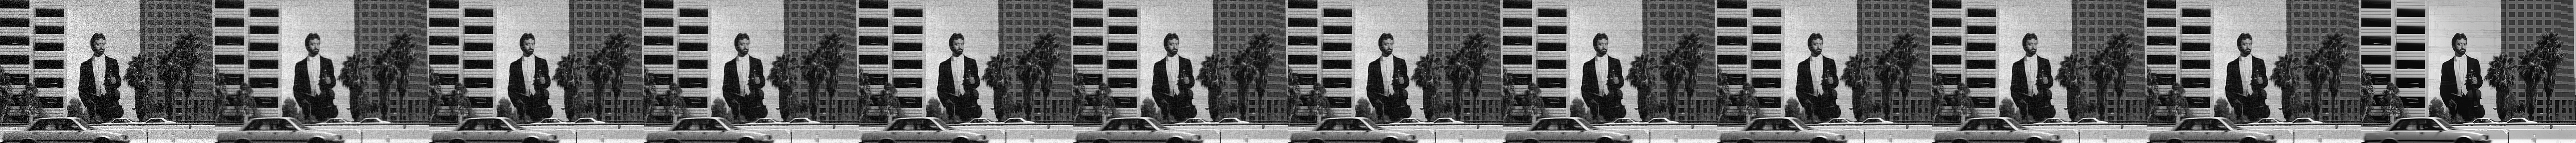
\includegraphics[width=\textwidth]{images/0004_stages.png}
\caption{Visual comparison of denoising results for $\sigma = 25$. Each row shows a strip consisting of the clean image (left), noisy observation (middle), and reconstructed outputs across stages (right).}
\label{fig:strip_results}
\end{figure*}

\subsection{Noise Model}

All experiments are conducted under additive Gaussian noise. Given a clean image $u$, the noisy observation $f$ is generated as
\begin{equation}
f = u + n,
\end{equation}
where $n \sim \mathcal{N}(0, \sigma^2)$ represents Gaussian noise with standard deviation $\sigma = 25$.

\subsection{Implementation Details}

The model is implemented using a multi-stage architecture derived from the discretized PDE. We use $T = 10$ stages and train each stage for 50 epochs. The number of filters is fixed across stages, and each filter has a kernel size of $7 \times 7$.

\subsection{Evaluation Metric}

We evaluate the denoising performance using the Peak Signal-to-Noise Ratio (PSNR):
\begin{equation}
\text{PSNR} = 10 \log_{10} \left( \frac{255^2}{\text{MSE}} \right).
\end{equation}

\section{Results}

\subsection{Quantitative Results}

We evaluate the performance of the proposed model on the CBSD68 dataset for a noise level of $\sigma = 25$. The model achieves an average PSNR of 26.29 dB when trained on the FOE400 dataset. This represents a significant improvement over classical PDE-based models. Table~\ref{tab:results} summarizes the comparison.

As shown in Fig.~\ref{fig:training_metrics}, the PSNR improves rapidly in the initial stages and gradually stabilizes, while the training loss decreases consistently, indicating stable convergence of the greedy training process.

\begin{table}[h]
\centering
\caption{Denoising Performance for $\sigma = 25$ on CBSD68}
\label{tab:results}
\begin{tabular}{l c}
\hline
Method & PSNR (dB) \\
\hline
Classical PDE & 18--20 \\
Proposed (BSD400) & 20.58 \\
Proposed (FOE400) & \textbf{26.29} \\
TNRD (reported) & 28--29 \\
\hline
\end{tabular}
\end{table}

\begin{figure}[h]
    \centering
    \begin{subfigure}{0.48\linewidth}
        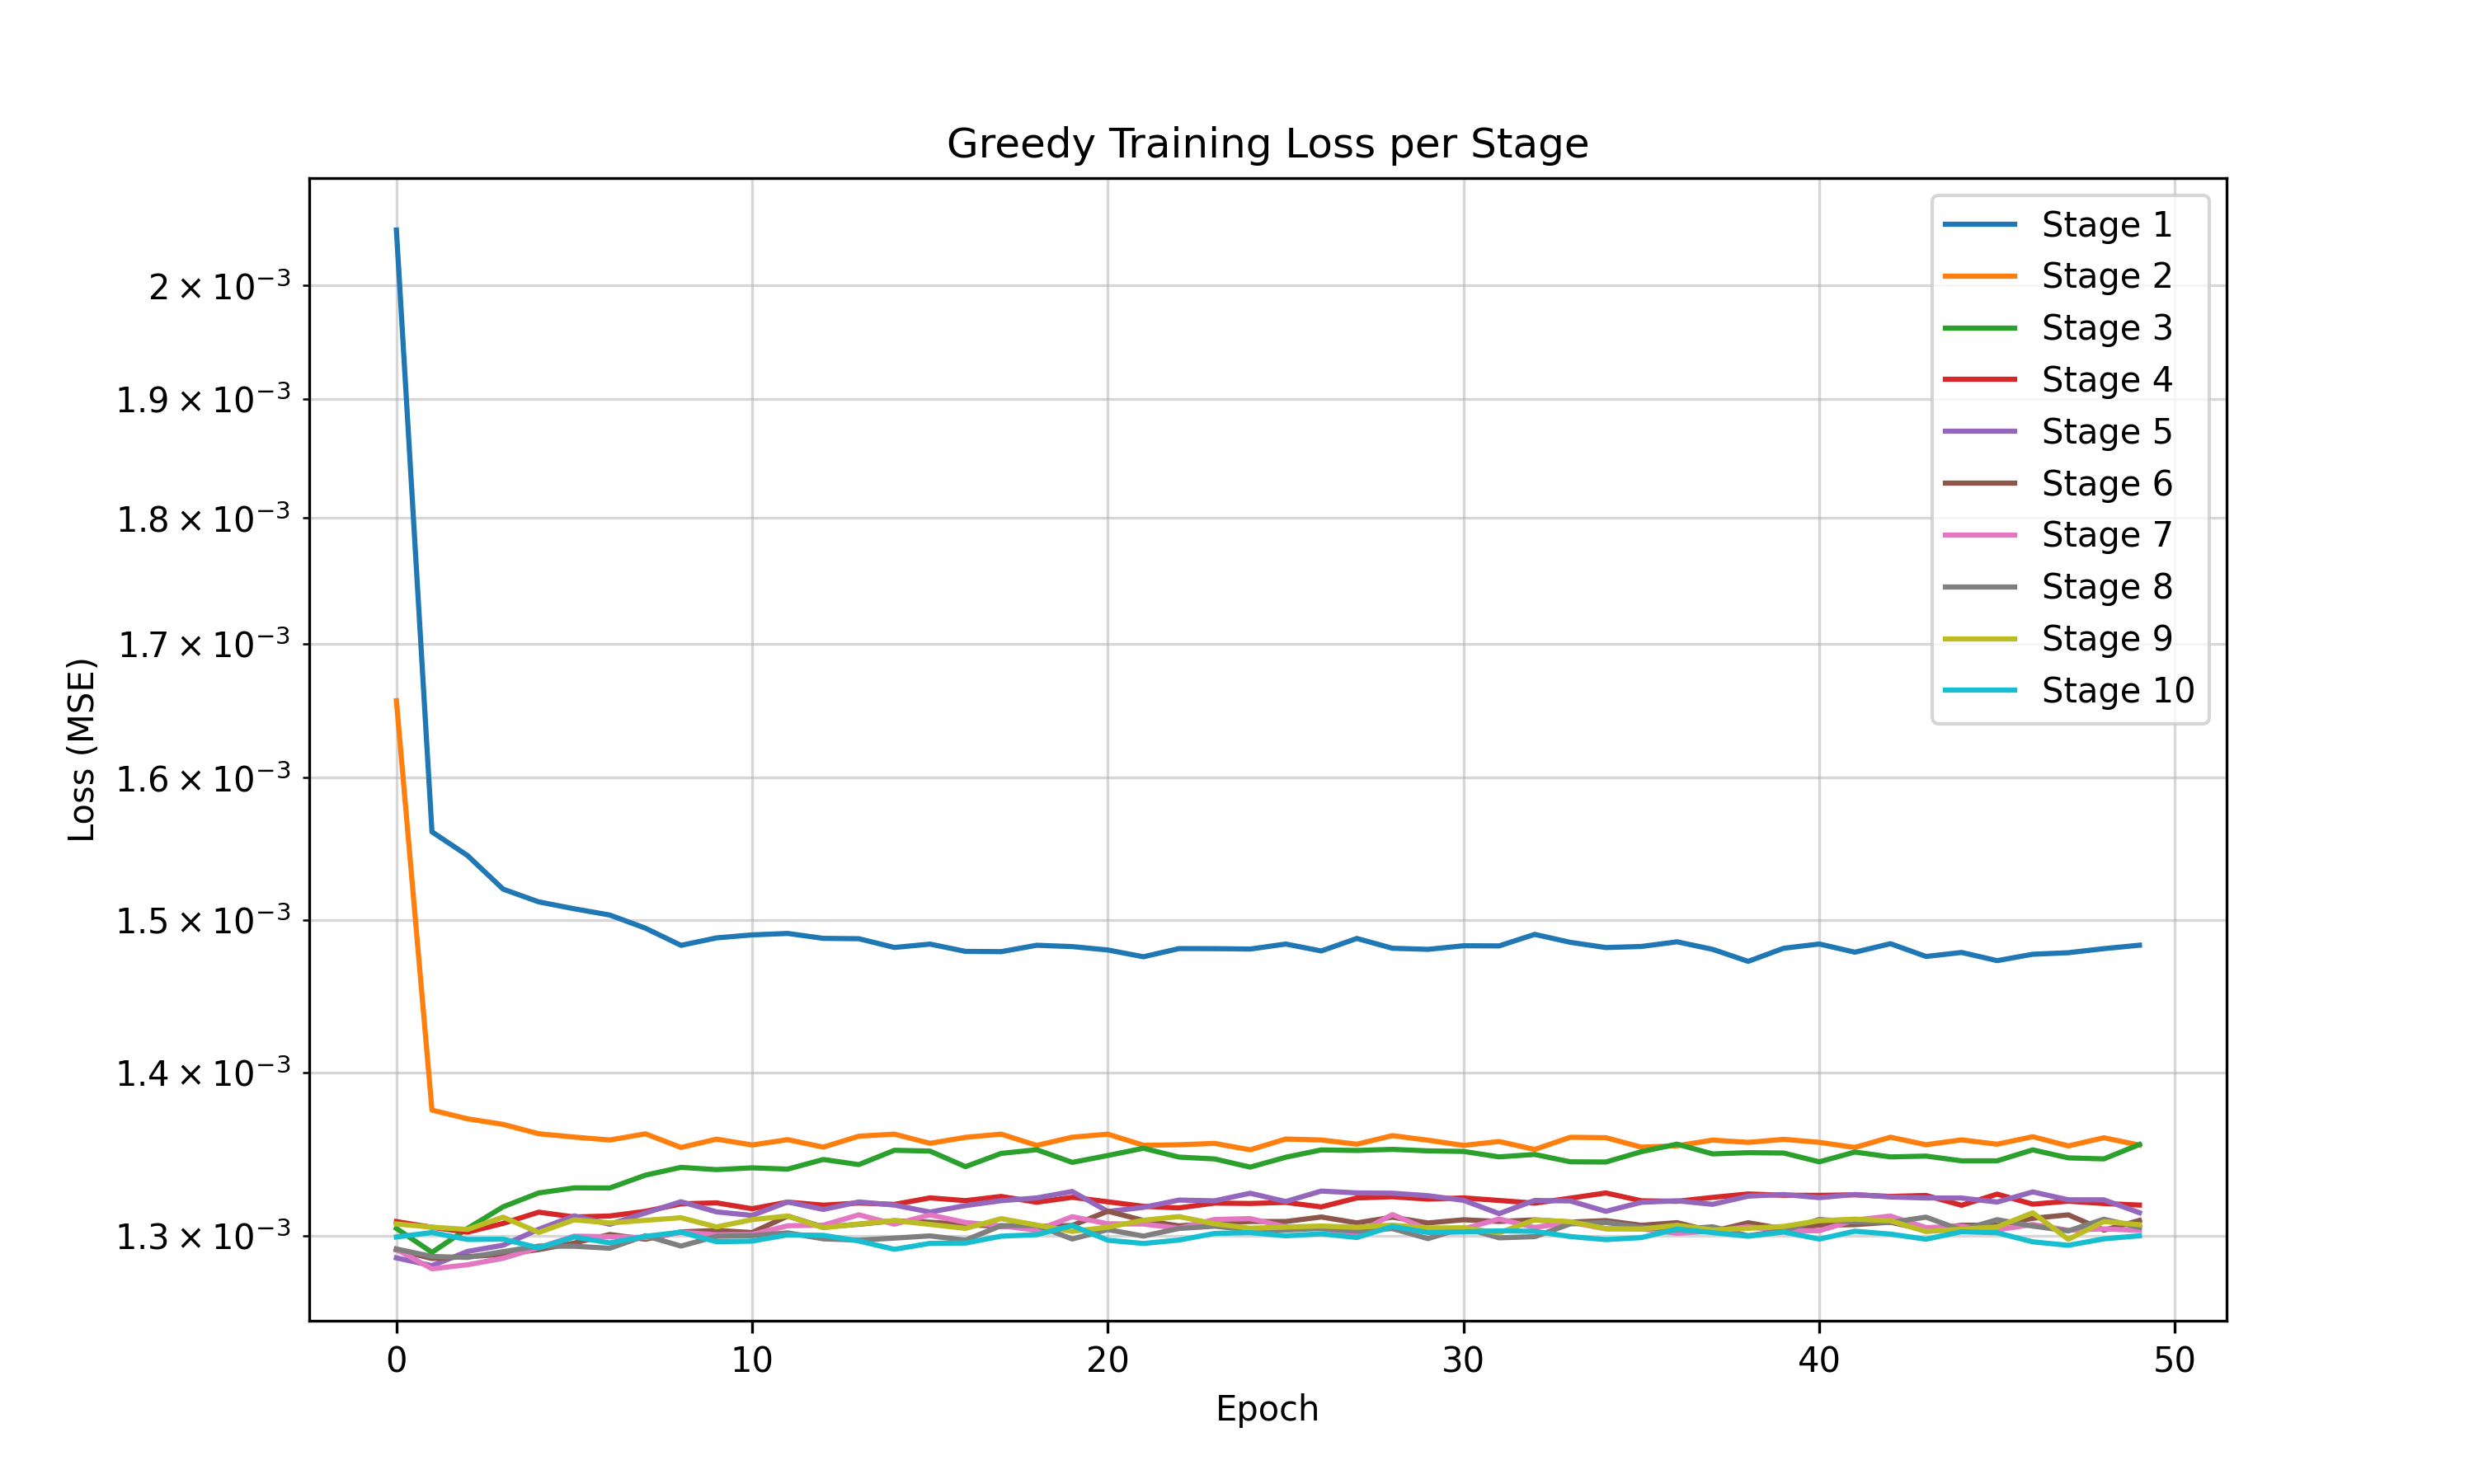
\includegraphics[width=\linewidth]{images/loss_plot.png}
        \caption{Loss per Stage}
        \label{fig:loss_plot}
    \end{subfigure}
    \hfill
    \begin{subfigure}{0.48\linewidth}
        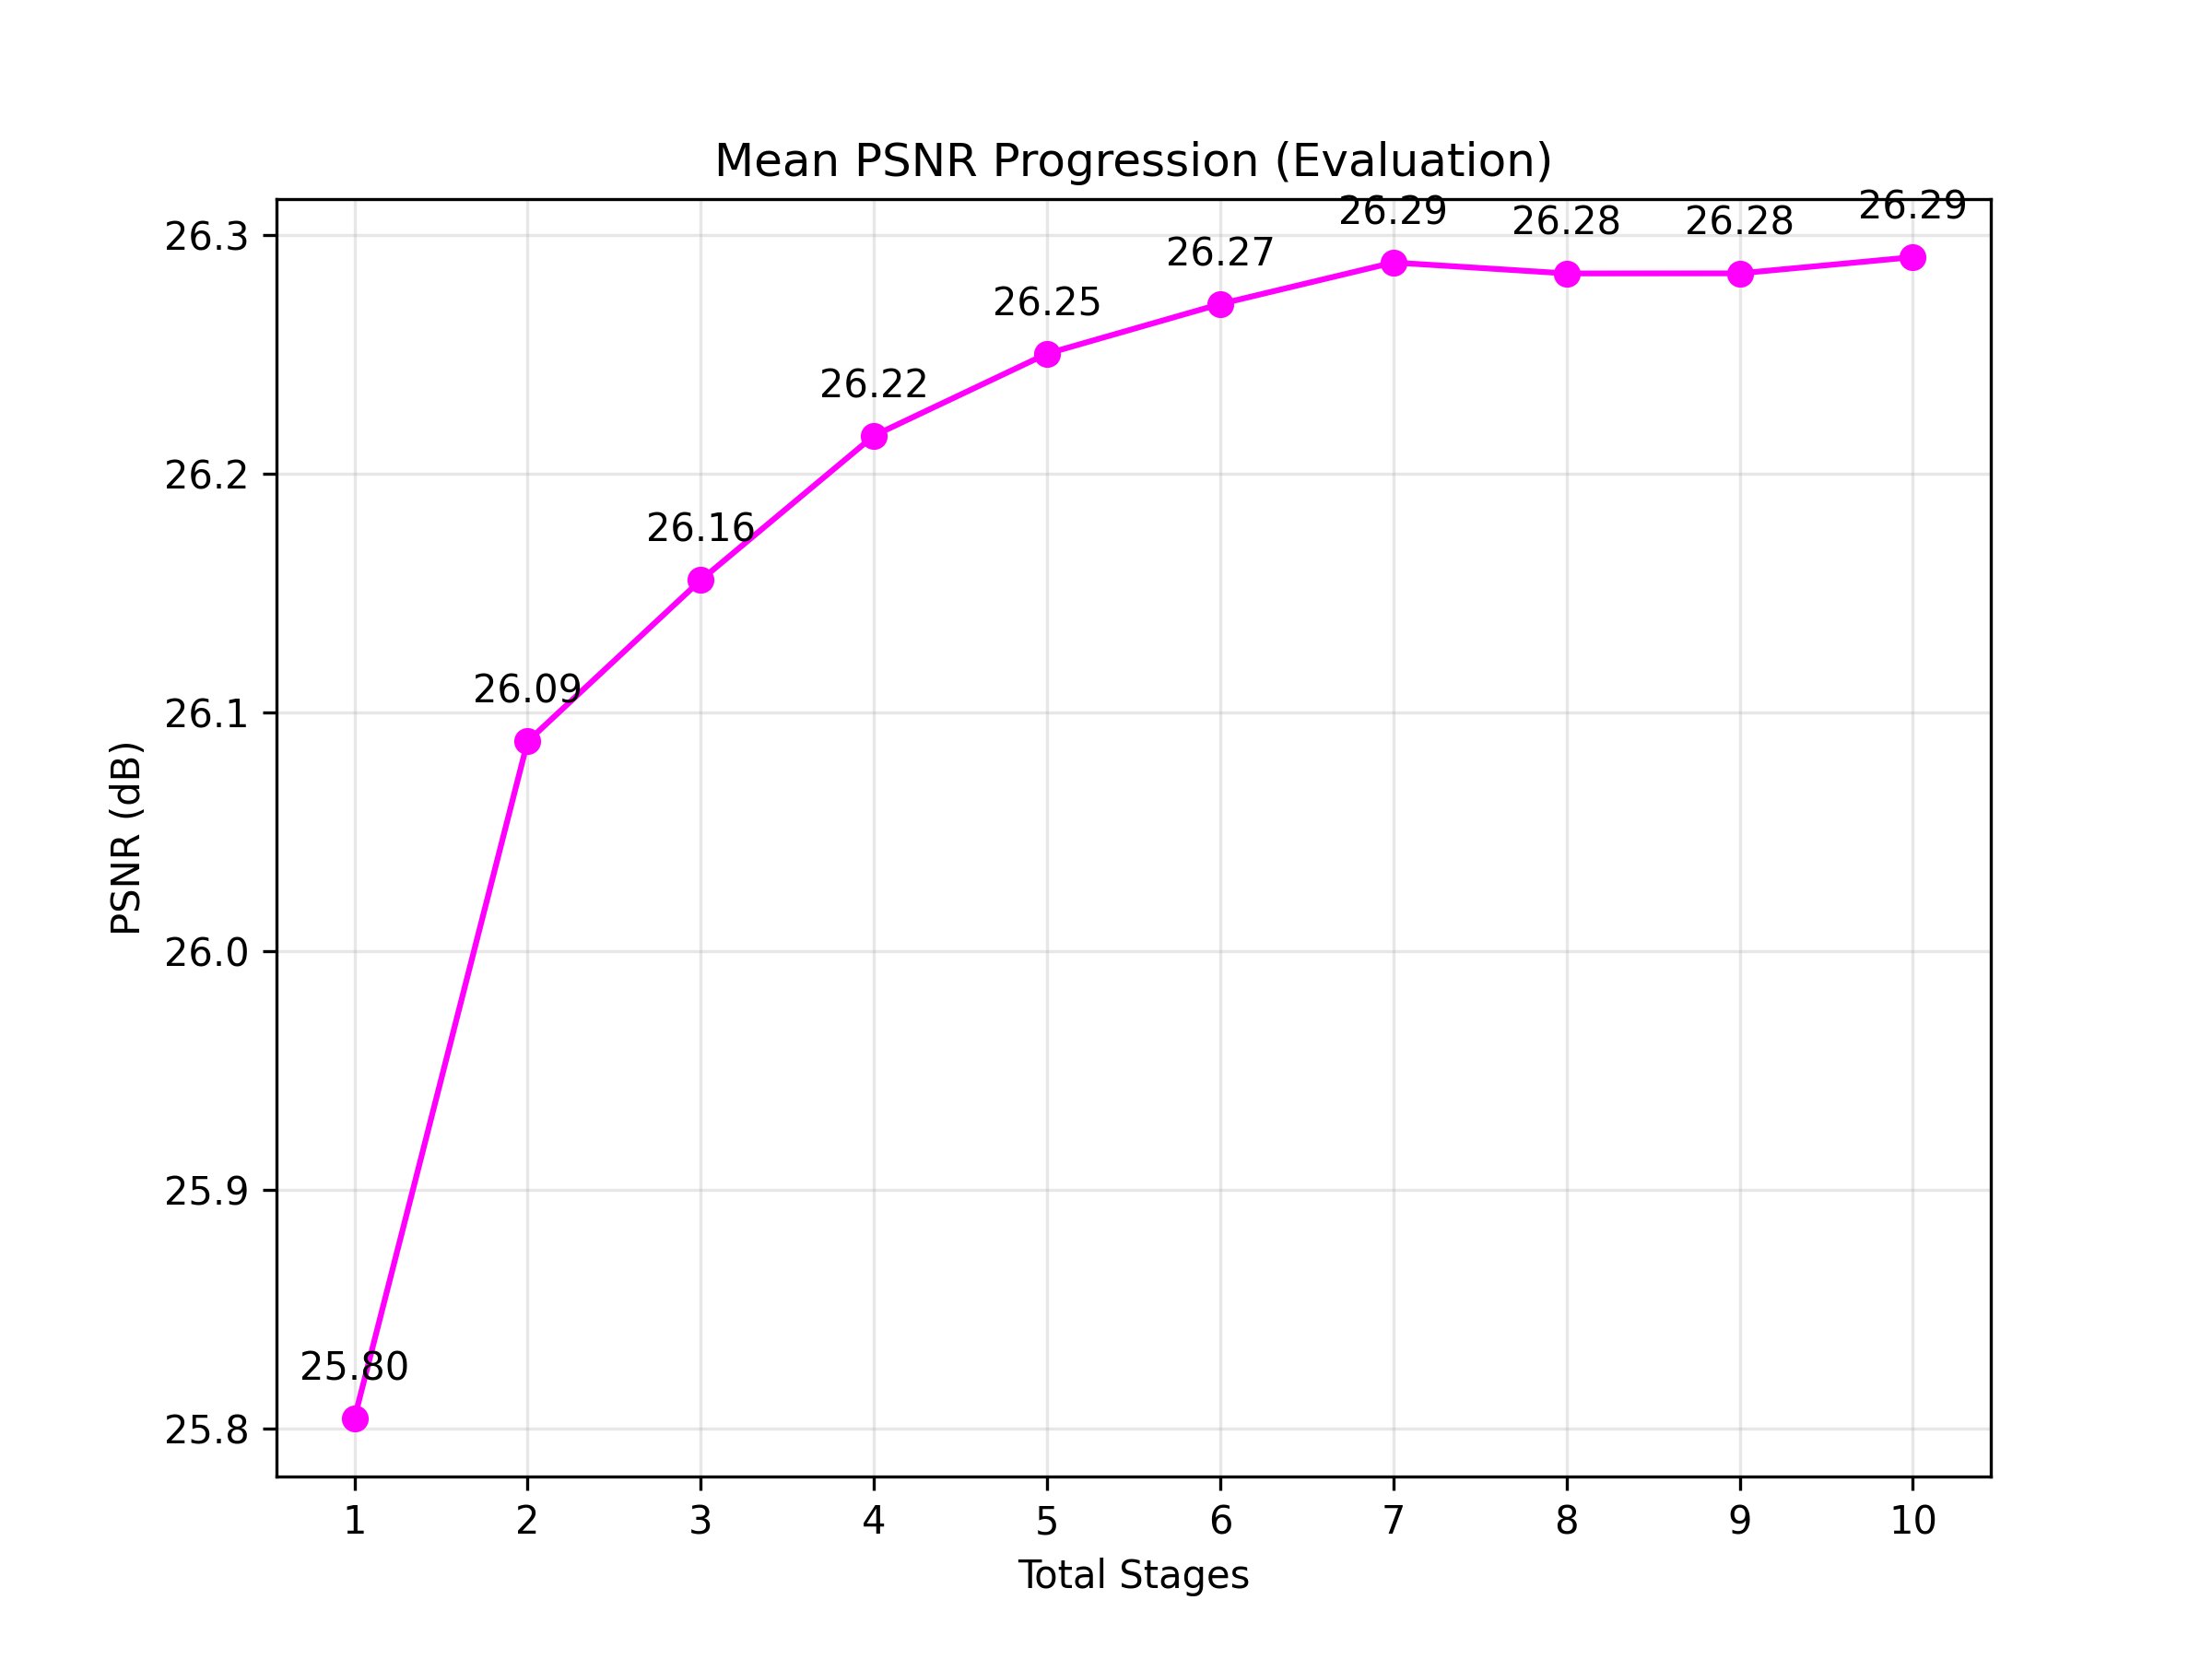
\includegraphics[width=\linewidth]{images/psnr_plot.png}
        \caption{PSNR Progression}
        \label{fig:psnr_plot}
    \end{subfigure}
    \caption{Training metrics: (a) MSE loss convergence per greedy stage, (b) Mean PSNR improvement as stages are added.}
    \label{fig:training_metrics}
\end{figure}

\begin{figure}[t]
\centering
% -------- Row 1 --------
\begin{subfigure}{0.3\linewidth}
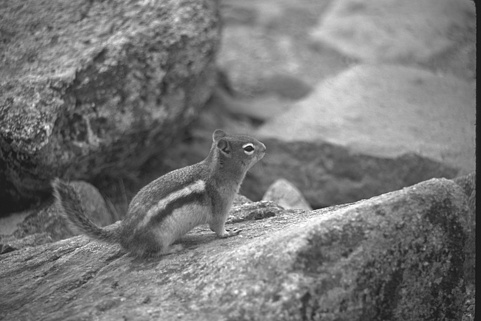
\includegraphics[width=\linewidth]{images/0000_clean.png}
\caption{0000 Clean}
\end{subfigure}
\hfill
\begin{subfigure}{0.3\linewidth}
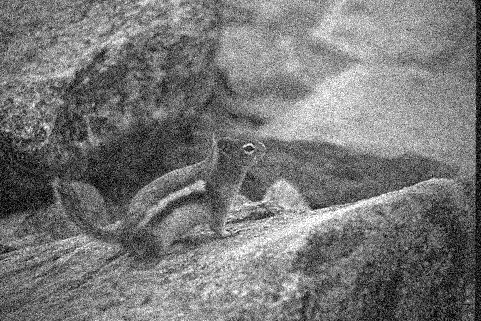
\includegraphics[width=\linewidth]{images/0000_noisy.png}
\caption{0000 Noisy}
\end{subfigure}
\hfill
\begin{subfigure}{0.3\linewidth}
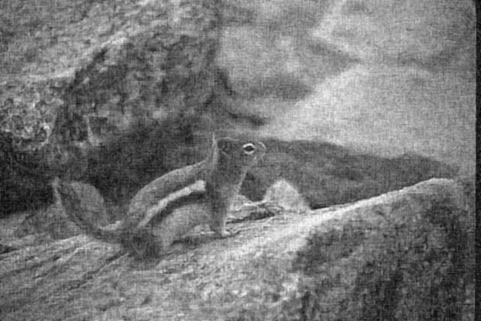
\includegraphics[width=\linewidth]{images/0000_denoised.png}
\caption{0000 Denoised}
\end{subfigure}
\vspace{0.4em}
% -------- Row 2 --------
\begin{subfigure}{0.3\linewidth}
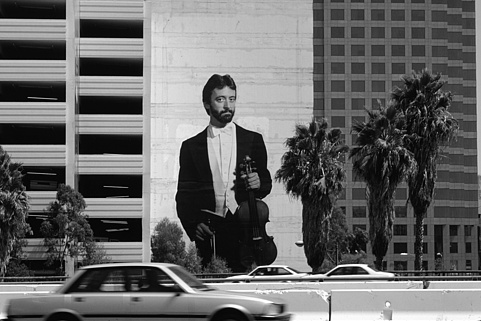
\includegraphics[width=\linewidth]{images/0004_clean.png}
\caption{0004 Clean}
\end{subfigure}
\hfill
\begin{subfigure}{0.3\linewidth}
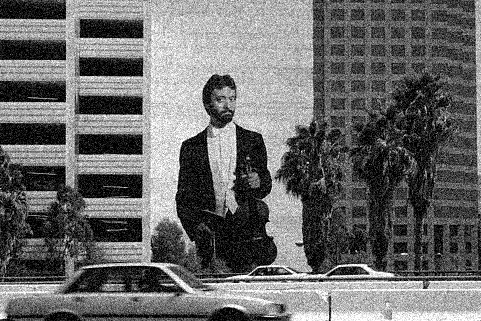
\includegraphics[width=\linewidth]{images/0004_noisy.png}
\caption{0004 Noisy}
\end{subfigure}
\hfill
\begin{subfigure}{0.3\linewidth}
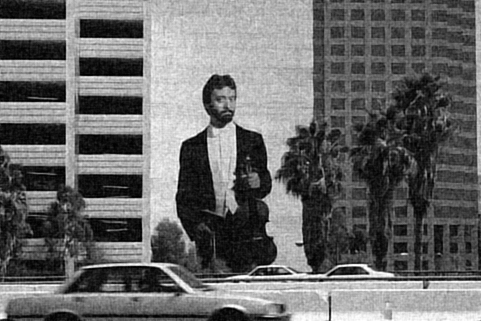
\includegraphics[width=\linewidth]{images/0004_denoised.png}
\caption{0004 Denoised}
\end{subfigure}
\vspace{0.4em}
% -------- Row 3 --------
\begin{subfigure}{0.3\linewidth}
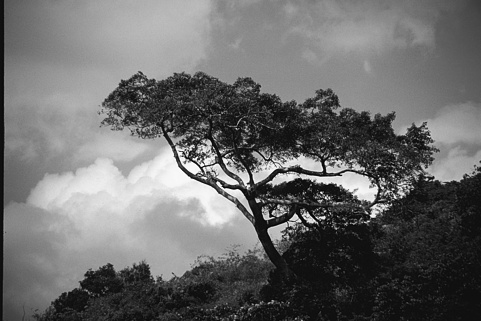
\includegraphics[width=\linewidth]{images/0002_clean.png}
\caption{0002 Clean}
\end{subfigure}
\hfill
\begin{subfigure}{0.3\linewidth}
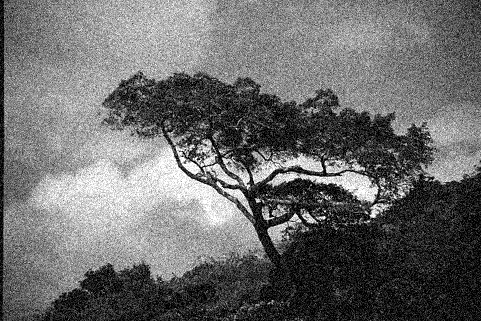
\includegraphics[width=\linewidth]{images/0002_noisy.png}
\caption{0002 Noisy}
\end{subfigure}
\hfill
\begin{subfigure}{0.3\linewidth}
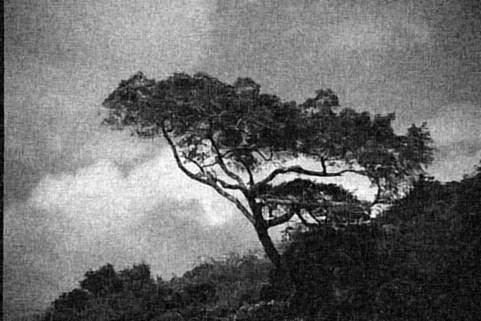
\includegraphics[width=\linewidth]{images/0002_denoised.png}
\caption{0002 Denoised}
\end{subfigure}
\caption{Denoising results for three samples (0000–0002). Each row shows clean, noisy, and reconstructed images.}
\label{fig:grid_results}
\end{figure}

Fig.~\ref{fig:grid_results} presents visual comparisons of clean, noisy, and reconstructed images, demonstrating that the proposed model effectively removes noise while preserving edges and fine details.

\subsection{Effect of Dataset}

We find that the selection of training dataset has a significant impact on performance. When trained on BSD400, the model achieves a PSNR of 20.58 dB. In contrast, training on the FOE400 dataset enhances the PSNR to 26.29 dB. This jump underscores the importance of utilizing diverse and representative training data for unrolled diffusion architectures.

\subsection{Stage-wise Analysis}

As shown in Fig.~\ref{fig:psnr_plot}, the most significant performance gains occur in the first few stages. The training loss also shows a steady convergence across all unrolled stages (Fig.~\ref{fig:loss_plot}). The PSNR starts at 25.80 dB at Stage 1 and gradually improves to 26.29 dB by Stage 10. Fig.~\ref{fig:strip_results} illustrates the progressive refinement of the denoised image across stages, showing how noise is gradually removed while preserving structural features.

\section{Discussion}

The experimental evidence shows that the proposed second-order formulation can learn meaningful denoising behavior and is significantly better than classical PDE-based methods. The introduction of second-order dynamics allows for faster refinement at the initial stages, as evidenced by the rapid rise in PSNR shown in Fig.~\ref{fig:psnr_plot}. This hyperbolic formulation introduces a "memory" component where each stage leverages information from the two preceding states, allowing for more fluid and effective diffusion.

While our model performs well, it does not yet reach the level of fully learned strategies like TNRD. This performance gap is likely due to our decision to fix the influence functions and damping coefficients, as well as the use of greedy stage-wise training. However, our architecture offers a more direct link to the underlying physics of the wave equation, providing better interpretability. The ability to achieve competitive results with fixed nonlinearities suggests that the second-order temporal structure itself carries significant expressive power. This approach could be used as a computationally efficient alternative to first-order models, especially in hardware-constrained environments where the number of unrolled steps needs to be minimized without sacrificing restoration quality.

\bibliographystyle{IEEEtran}
\bibliography{references}

\end{document}